\documentclass[notheorems, handout]{beamer}
	
\usefonttheme[onlymath]{serif}
\setbeamertemplate{navigation symbols}{}

	
\usepackage[utf8]{inputenc}
\usepackage[T2A]{fontenc}
\usepackage[russian]{babel}
\usepackage{tikz}
\usepackage{ragged2e}
\usepackage{amsthm}
\usepackage{wrapfig}
\usepackage{bm} %bold math
\usepackage{url}	
\usepackage{graphicx}
\usepackage{marginnote}
\usepackage{bm}
\usepackage[makeroom]{cancel}
\usepackage{algorithm2e}
\setbeamertemplate{navigation symbols}{}
\setbeamertemplate{footline}[frame number]

\newcommand{\sign}{\text{sign}}
\DeclareMathOperator*{\argmax}{arg\,max}
\DeclareMathOperator*{\argmin}{arg\,min}
\DeclareMathOperator{\rank}{rank}
\DeclareMathOperator{\diam}{diam}
\DeclareMathOperator{\ob}{Ob}
\DeclareMathOperator{\Hom}{Hom}
\DeclareMathOperator{\var}{Var}
\DeclareMathOperator{\bias}{Bias}
\newcommand{\betah}{\hat{\bm \beta}}
\newcommand{\betaa}{\bm{\beta}}
\newcommand{\epss}{\bm{\varepsilon}}
\newcommand{\E}{\mathrm{E}}
\newcommand{\D}{\mathrm{D}}
\newcommand{\XT}{{\bm{X}}^{\mathrm{T}}}
\newcommand{\X}{\bm{X}}
\renewcommand{\thealgocf}{}
\definecolor{asparagus}{rgb}{0.53, 0.66, 0.42}
	
\newtheorem{theorem}{Теорема}
\newtheorem{definition}{Определение}
\addto\captionsrussian{\renewcommand{\figurename}{Figure}}
\addto\captionsrussian{\renewcommand{\tablename}{Table}}
	
\title[Neural Nets (NN), глубокое обучение, рекуррентные сети, LSTM и пр. Работа с временными рядами (прогноз) и с текстами. Трансформеры, BERT]{%
	    Neural Nets (NN), глубокое обучение, рекуррентные сети, LSTM и пр. Работа с временными рядами (прогноз) и с текстами. Трансформеры, BERT}
	
\author[Оленев Роман, Самарин Игорь]{Оленев Роман, Самарин Игорь}
%\textsc{}
	
\institute[Санкт-Петербургский Государственный Университет]{%
	    \small
	    Санкт-Петербургский государственный университет\\
	    Кафедра статистического моделирования\\
	    \vspace{1.25cm}
	}
	
\date[]{Санкт-Петербург, 2024}
	
%\subject{Talks}
	
\begin{document}
	
	\begin{frame}[plain]
		\titlepage
	\end{frame}
	
	
	\begin{frame}
	\frametitle{NLP}
		Обработка текстов на естественном языке (Natural Language Processing, NLP) --- общее направление искусственного интеллекта и математической лингвистики. Оно изучает проблемы компьютерного анализа и синтеза текстов на естественных языках.
		
		Подходы к представлению текста:
		\begin{enumerate}
			\item Bag of words
			\item Bag of Ngramms
			\item TF-IDF
			\item Word Embeddings
		\end{enumerate}
	\end{frame}
	
	\begin{frame}
	\frametitle{Word2Vec}
		\begin{figure}[H]
			\begin{center}
				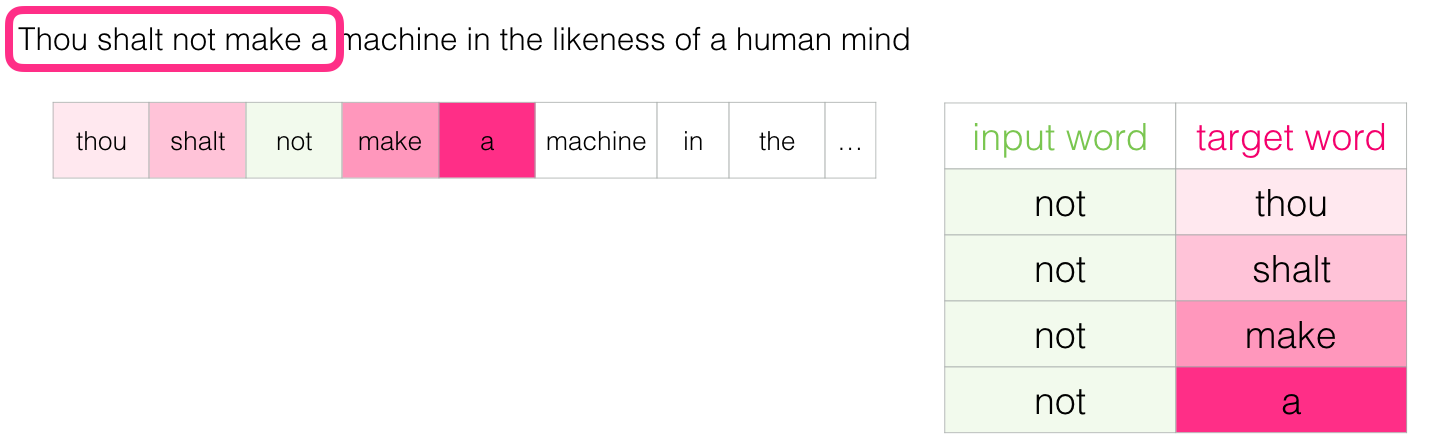
\includegraphics[scale=0.15]{img/skip-gram.png}
				\caption{SkipGram}
			\end{center}
		\end{figure}
		
		\begin{figure}[H]
			\begin{center}
				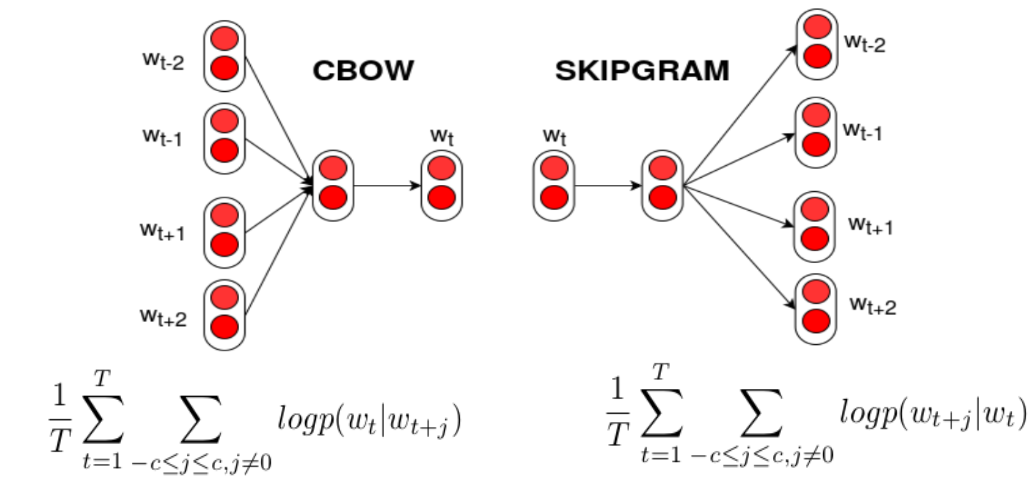
\includegraphics[scale=0.35]{img/word2vec.png}
				\caption{Word2Vec}
			\end{center}
		\end{figure}
	\end{frame}
	
	\begin{frame}
	\frametitle{Машинный перевод. Постановка задачи}
		Пусть есть входная последовательность $x_1, x_2, \dots, x_m$ и выходная последовательность $y_1, y_2, \dots, y_n$. Тогда хотим максимизировать $p(y|x)$: $y^{\ast}=\arg\max\limits_{y}p(y|x).$
		\vspace{0.3cm}
		\begin{figure}[H]
			\begin{center}
				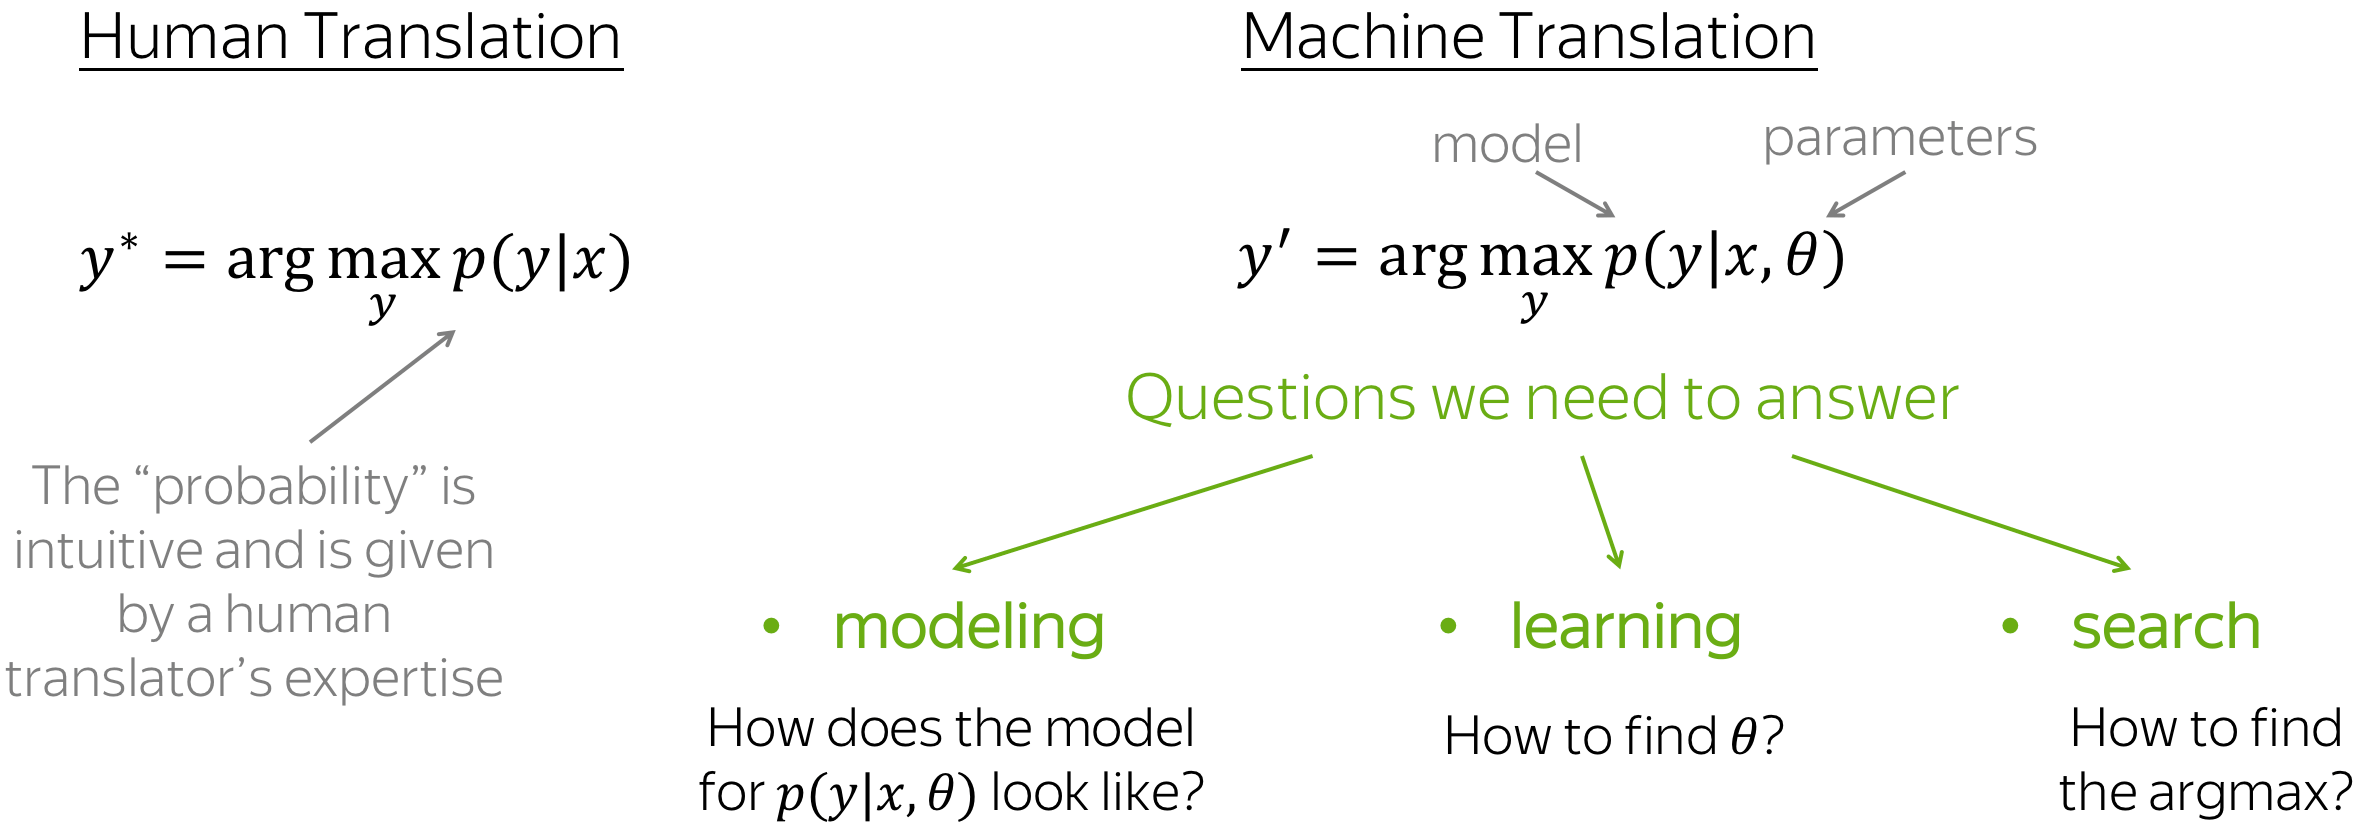
\includegraphics[scale=0.1]{img/translation.png}
			\end{center}
		\end{figure}
	\end{frame}
	
	\begin{frame}
	\frametitle{Машинный перевод. 2 RNNs}
		\begin{figure}[H]
			\begin{center}
				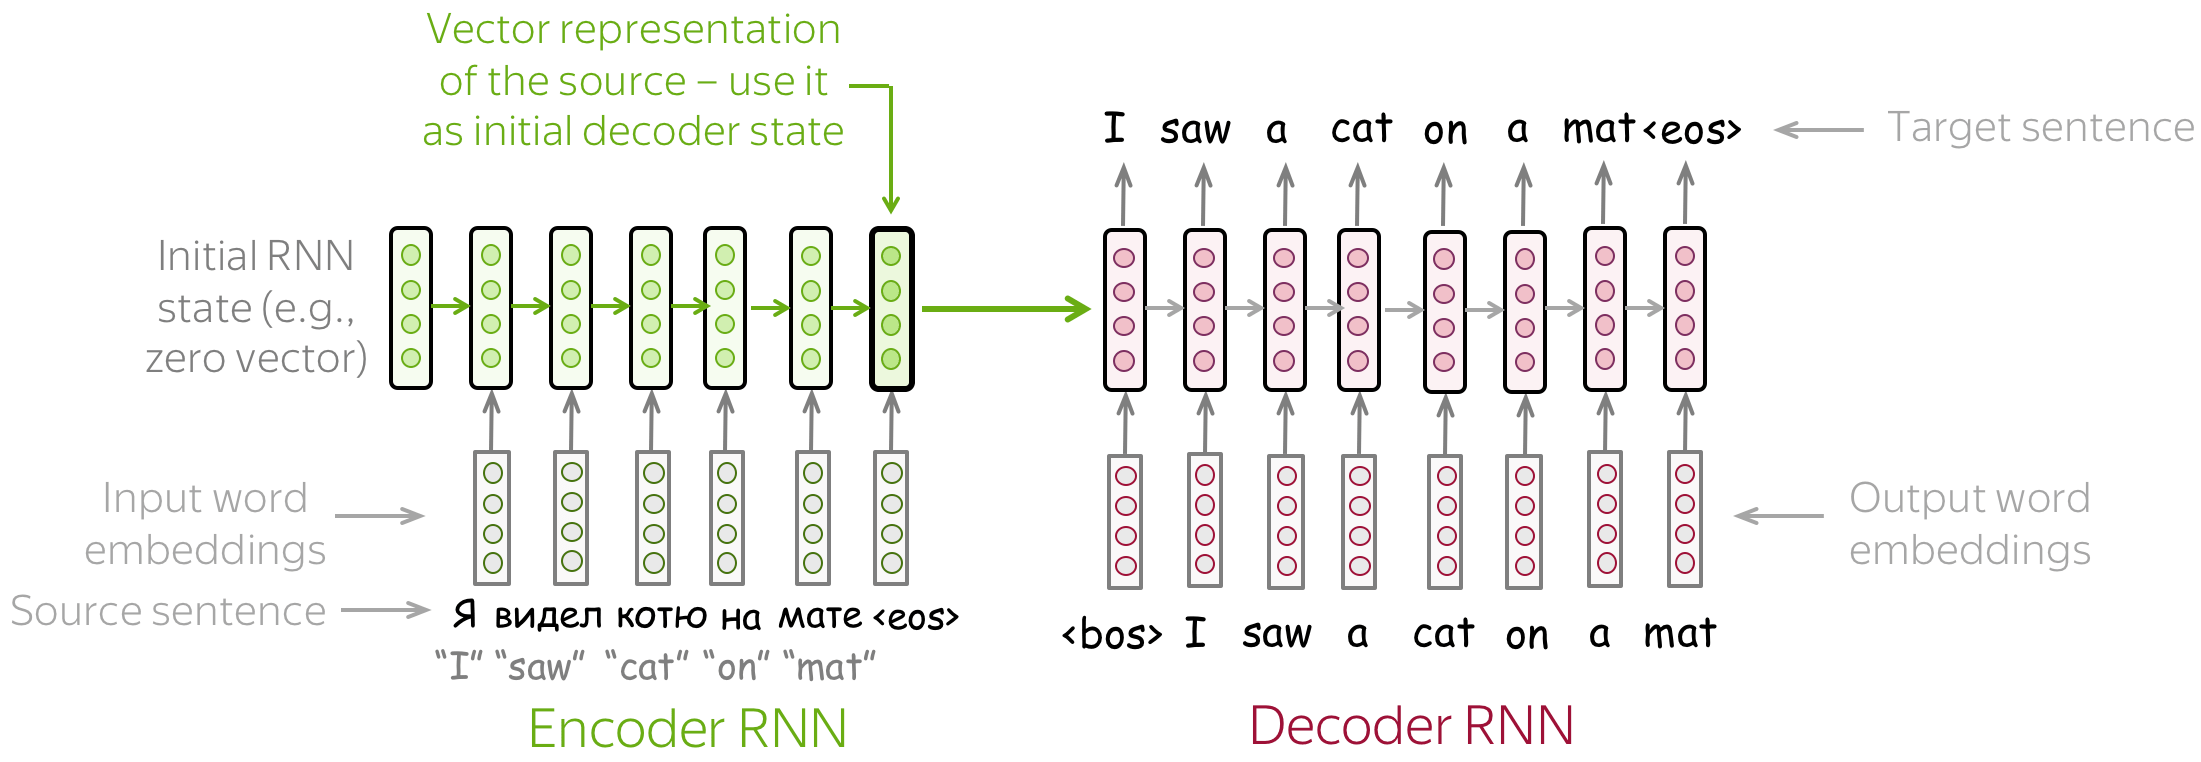
\includegraphics[scale=0.1]{img/two_rnn.png}
			\end{center}
		\end{figure}

		\begin{figure}[H]
			\begin{center}
				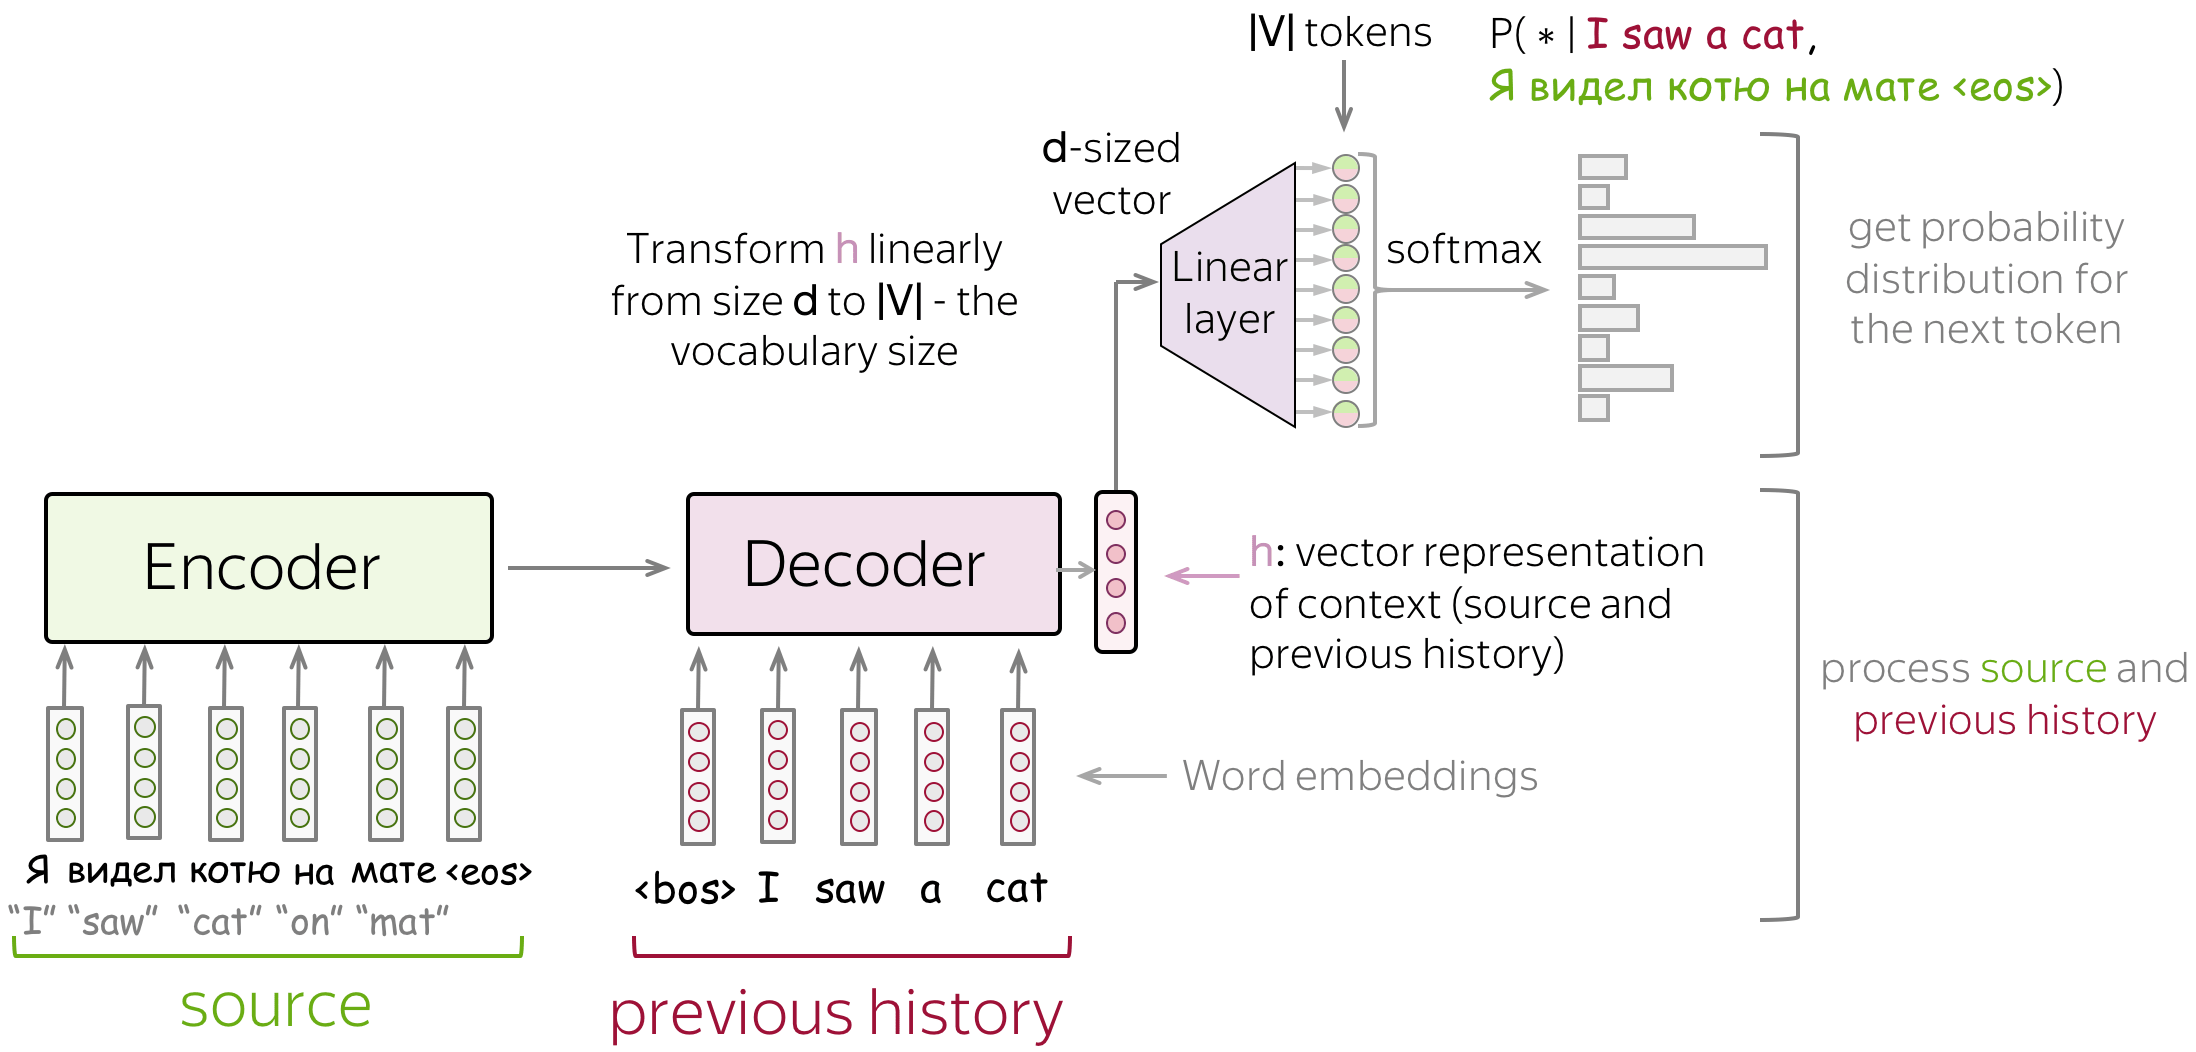
\includegraphics[scale=0.1]{img/two_rnn2.png}
			\end{center}
		\end{figure}
	\end{frame}
	\begin{frame}
	\frametitle{Машинный перевод. Обучение и предсказание}
		В качестве функции потерь используется кросс--энтропия. При обучении на вход случайным образом можно подавать не только предсказанное на предыдущем шаге слово, но и верное слово.
	
		$Loss(p^{\ast}, p^{})= - p^{\ast} \log(p) = -\sum\limits_{i=1}^{|V|}p_i^{\ast} \log(p_i).$
		$Loss(p^{\ast}, p) = -\log(p_{y_t})=-\log(p(y_t| y_{\mbox{<}t}, x)).$
		\vspace{0.3cm}
		
	 	Прогноз:
	 	\begin{enumerate}
	 		\item Greedy Decoding (предсказываем самое вероятное)
	 		\item Beam Search (на каждом шаге храним несколько вероятных последовательностей)
	 	\end{enumerate}
	\end{frame}
		
	\begin{frame}
	\frametitle{Механизм Attention}
		Проблема: невозможно сохранить весь контекст в одном векторе. Решением проблемы является механизм внимания.
		\begin{figure}[H]
			\begin{center}
				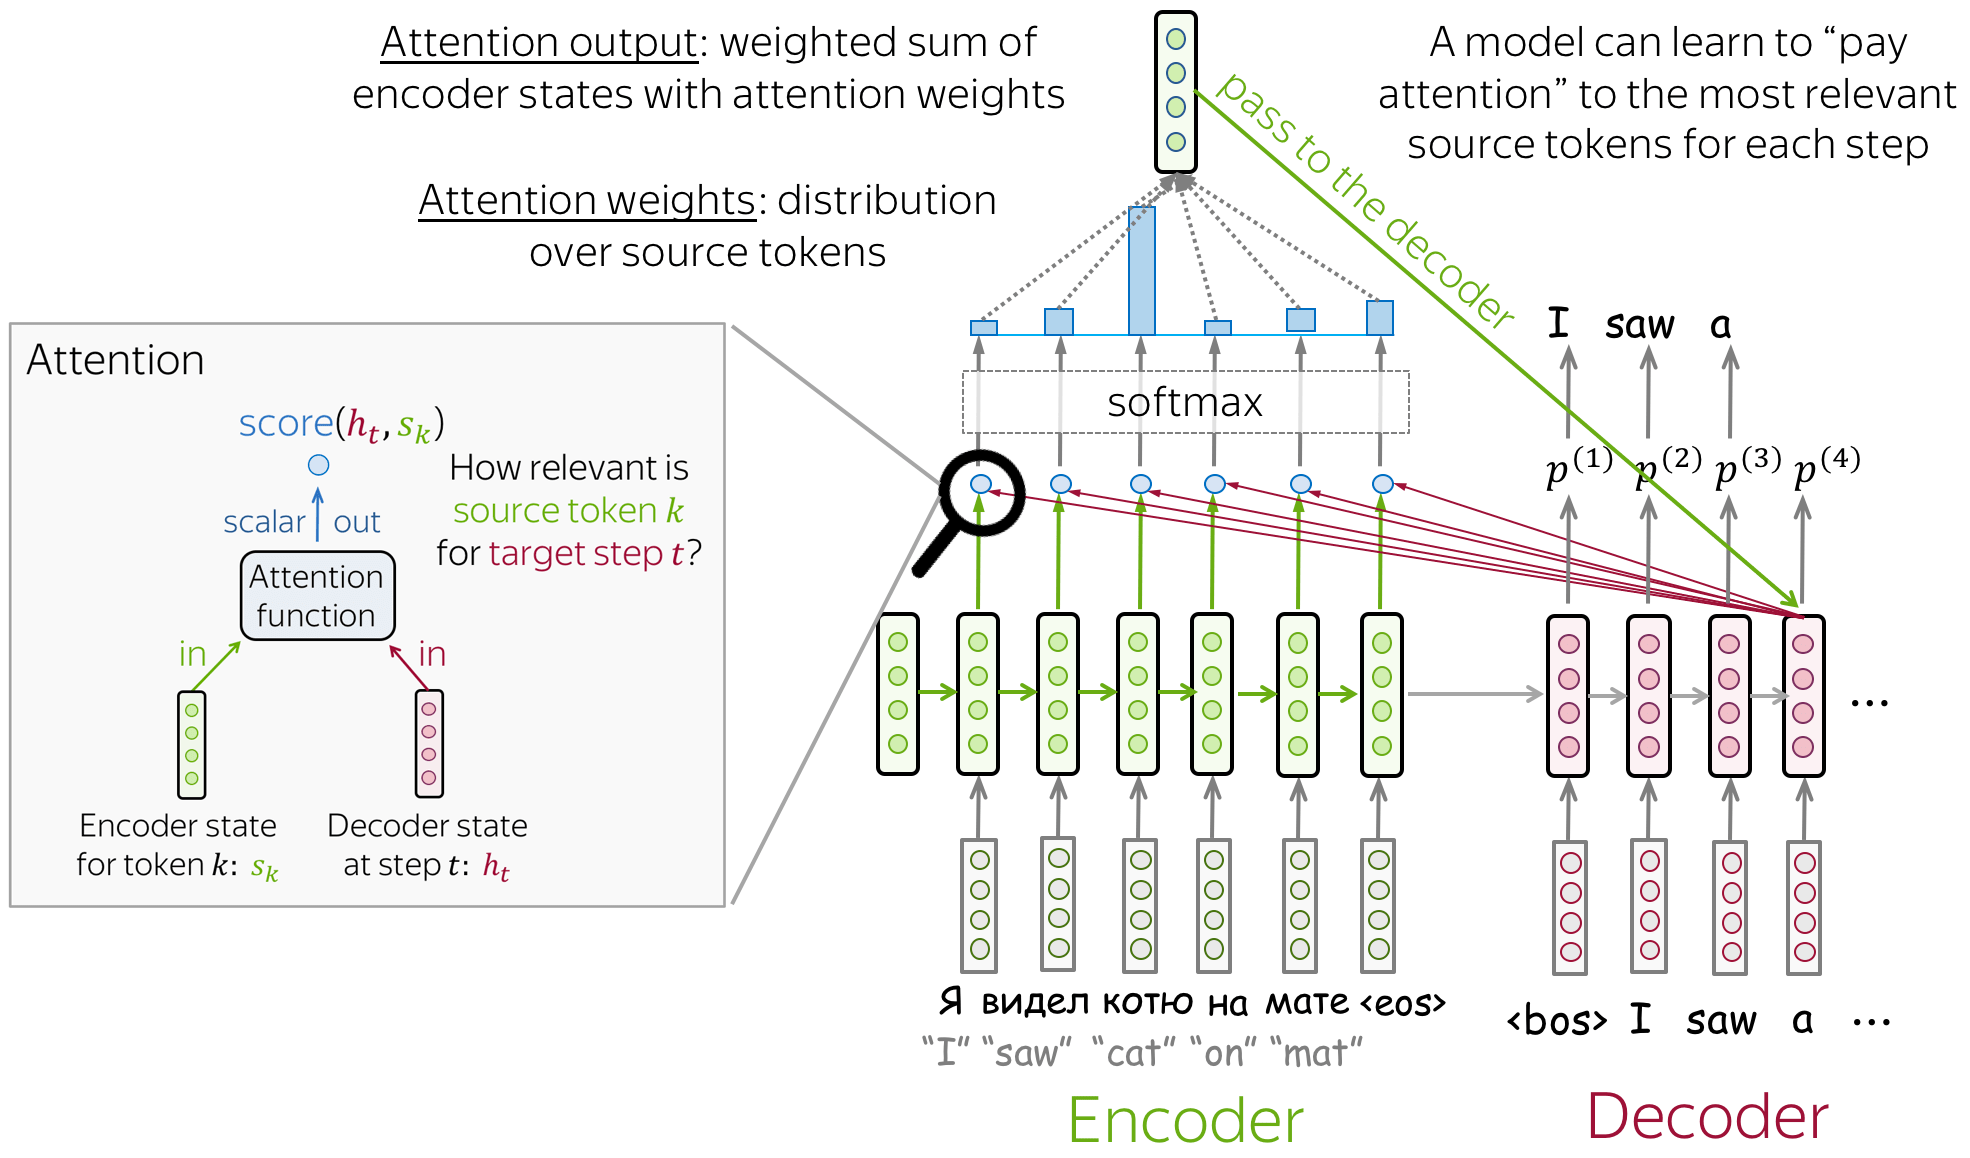
\includegraphics[scale=0.15]{img/general_scheme_att.png}
			\end{center}
		\end{figure}		
	\end{frame}
	
	\begin{frame}
	\frametitle{Механизм Attention}
		\begin{figure}[H]
			\begin{center}
				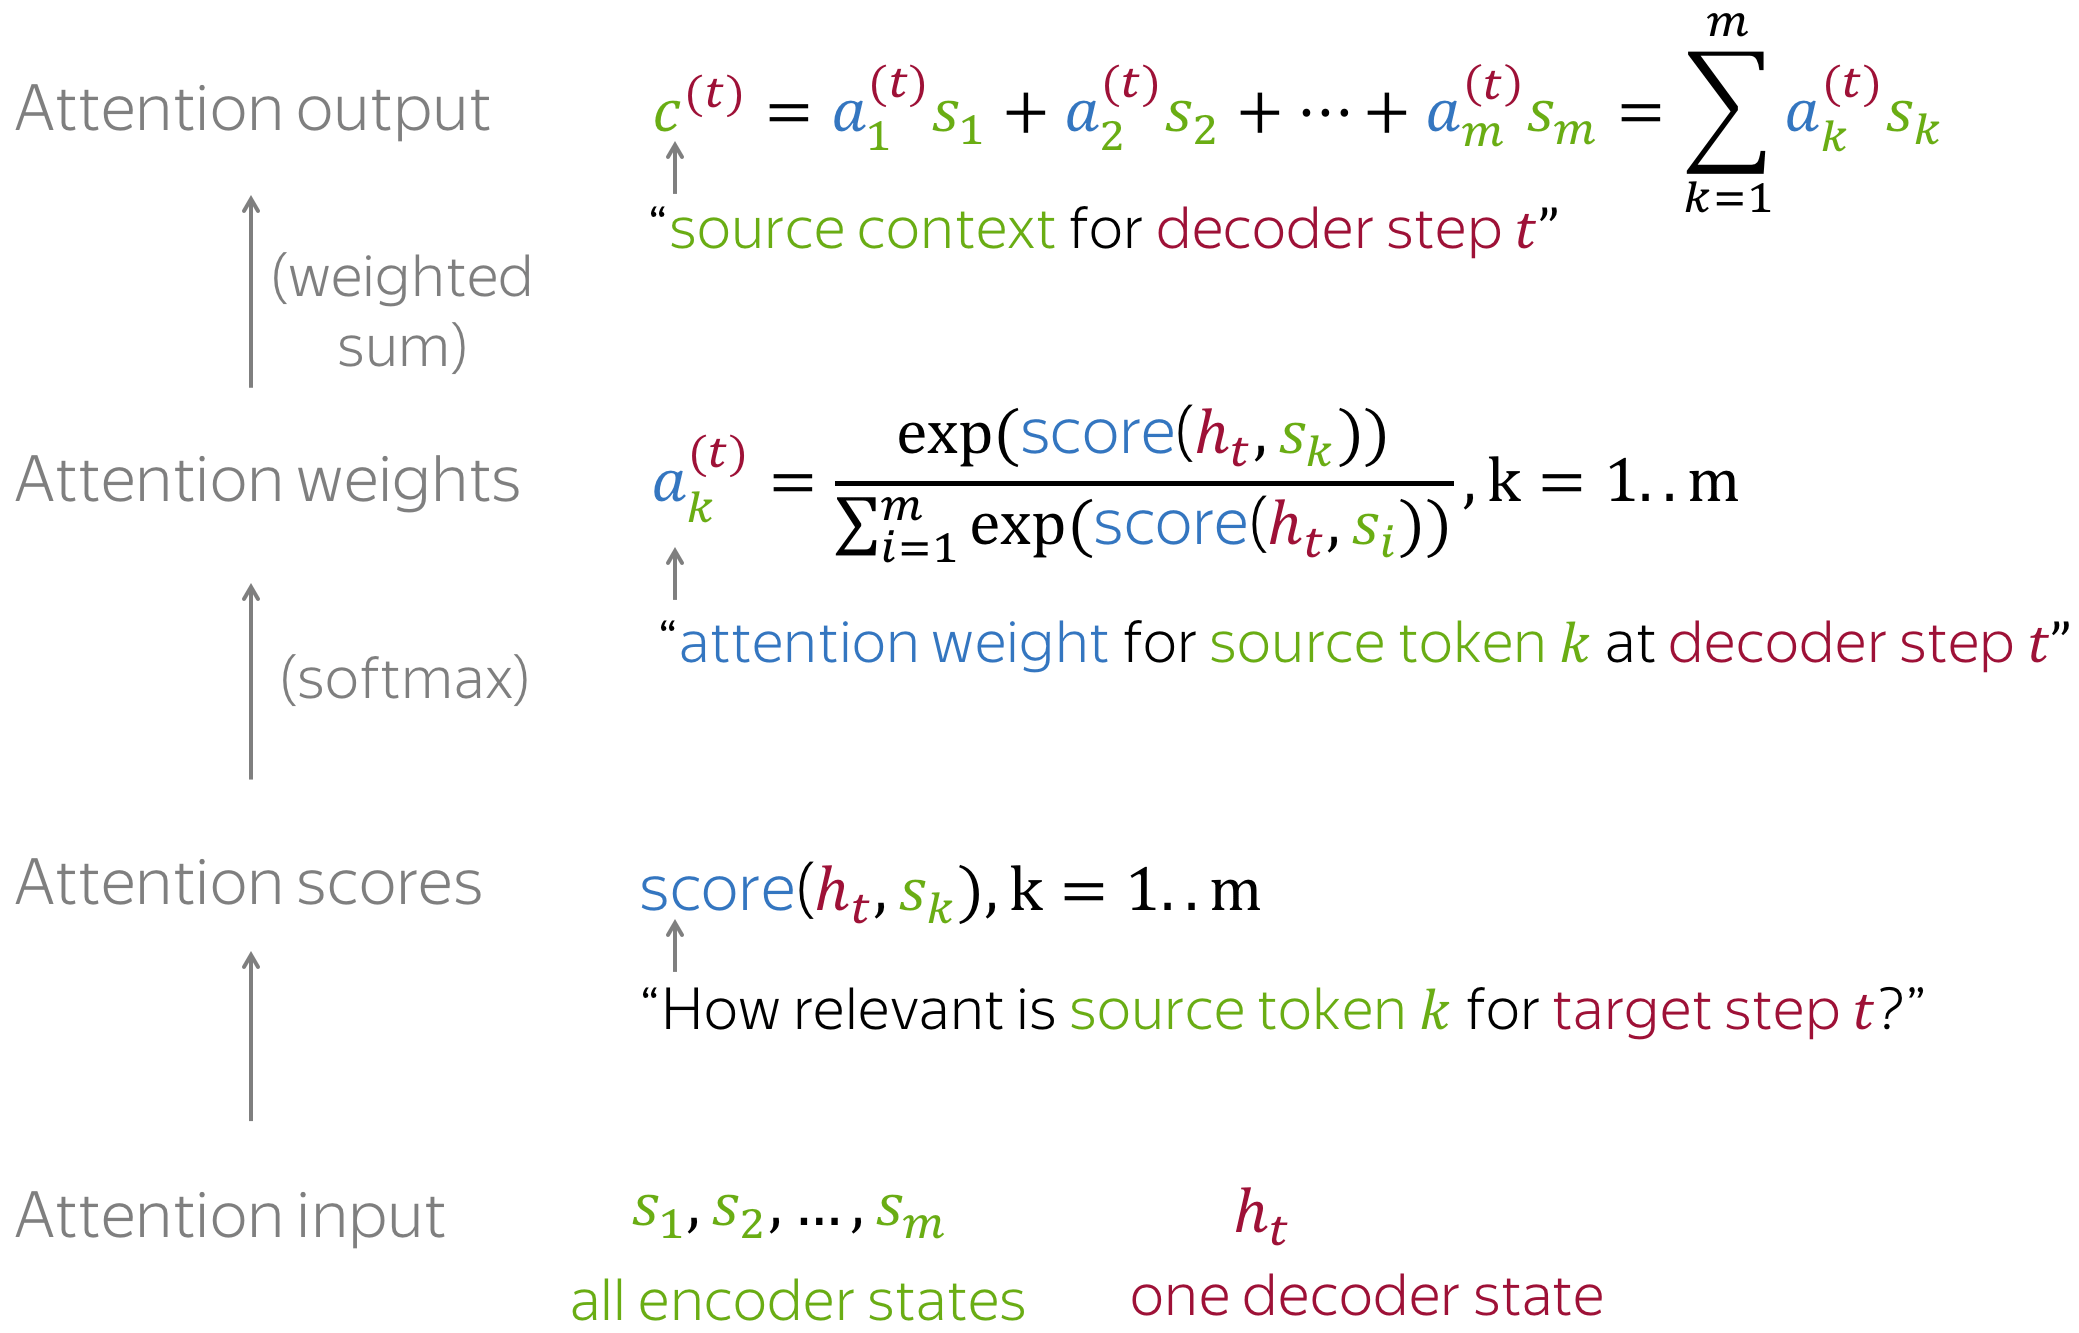
\includegraphics[scale=0.1]{img/att.png}
			\end{center}
		\end{figure}
		\begin{figure}[H]
			\begin{center}
				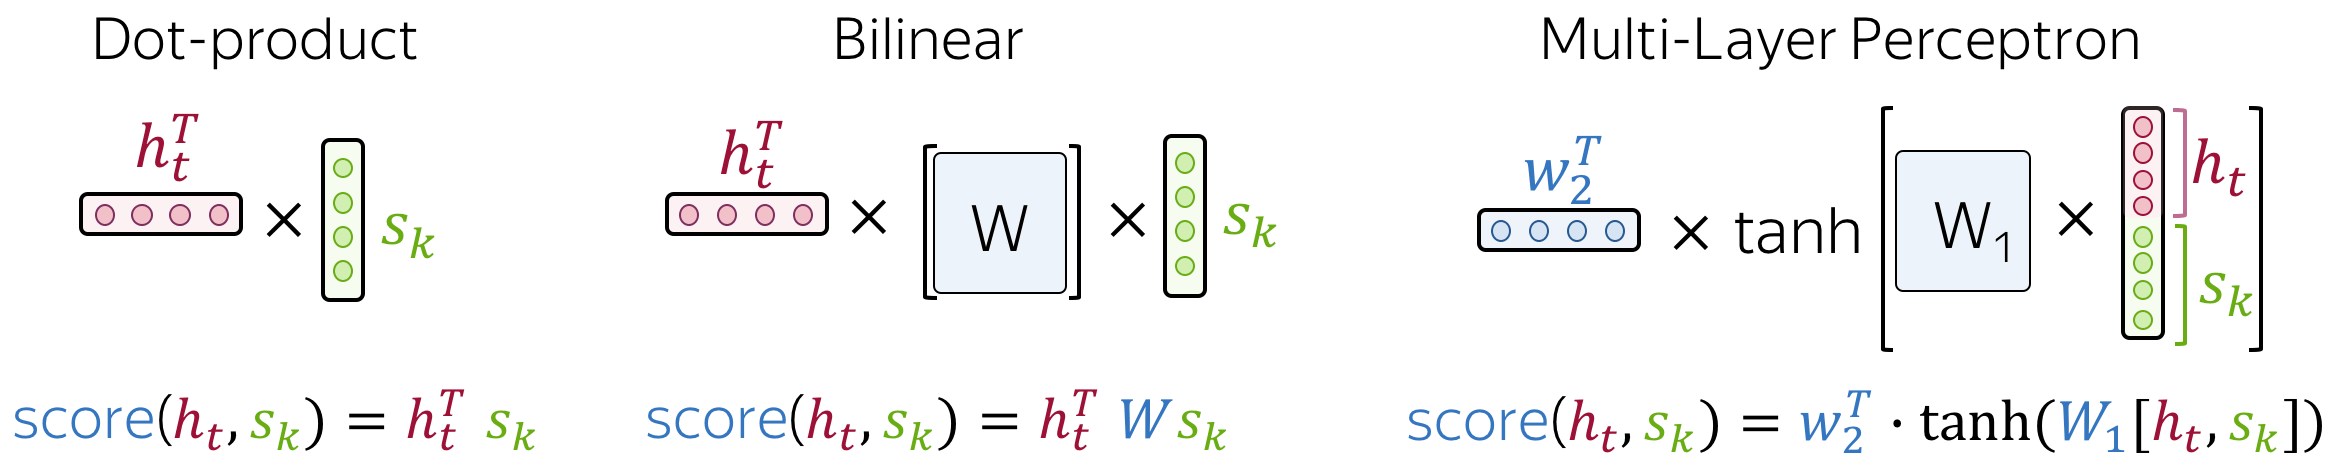
\includegraphics[scale=0.1]{img/att2.png}
			\end{center}
		\end{figure}
	\end{frame}
	
	\begin{frame}
	\frametitle{Трансформеры}
		\begin{figure}[H]
			\begin{center}
				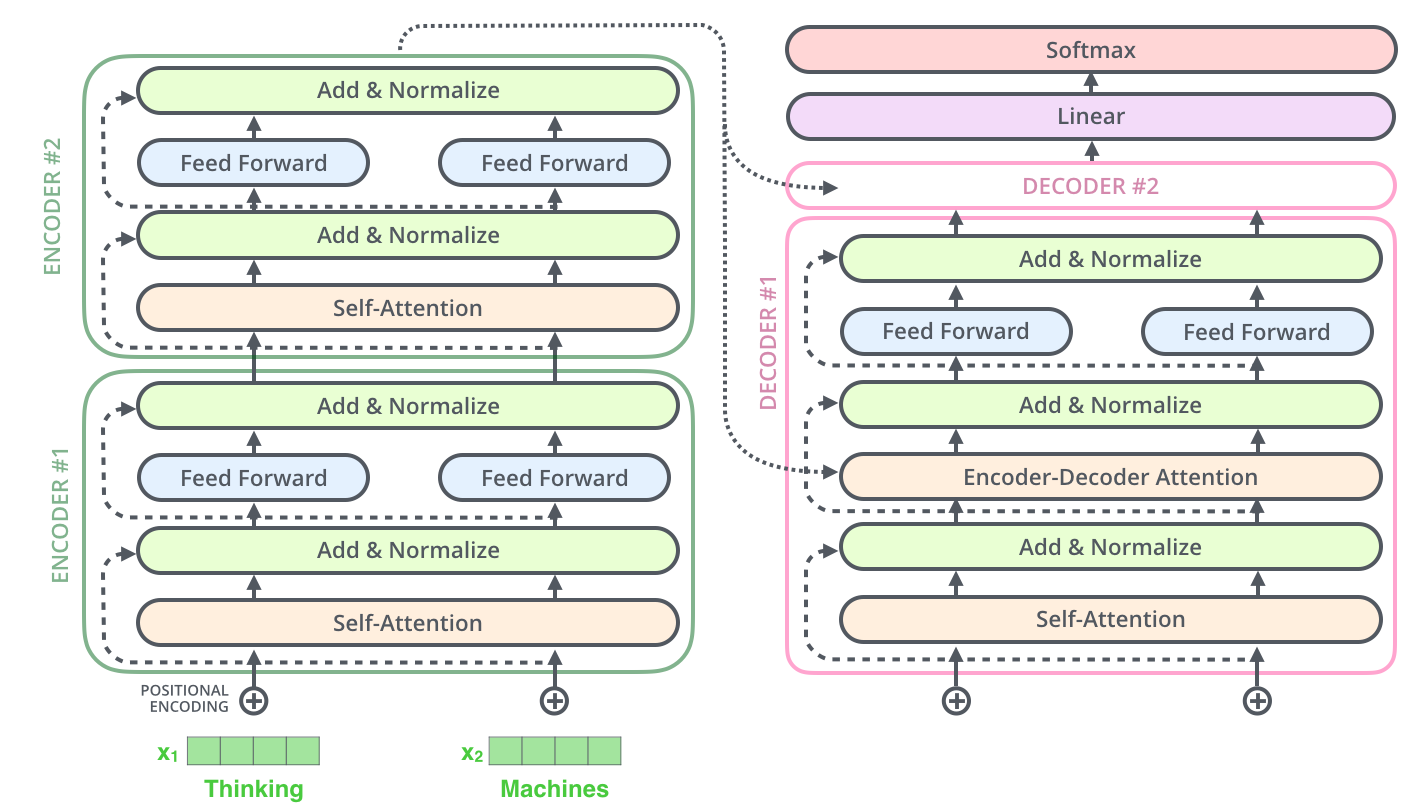
\includegraphics[scale=0.12]{img/transf.png}
				\caption{Архитектура Трансформер}
			\end{center}
		\end{figure}
		\begin{figure}[H]
			\begin{center}
				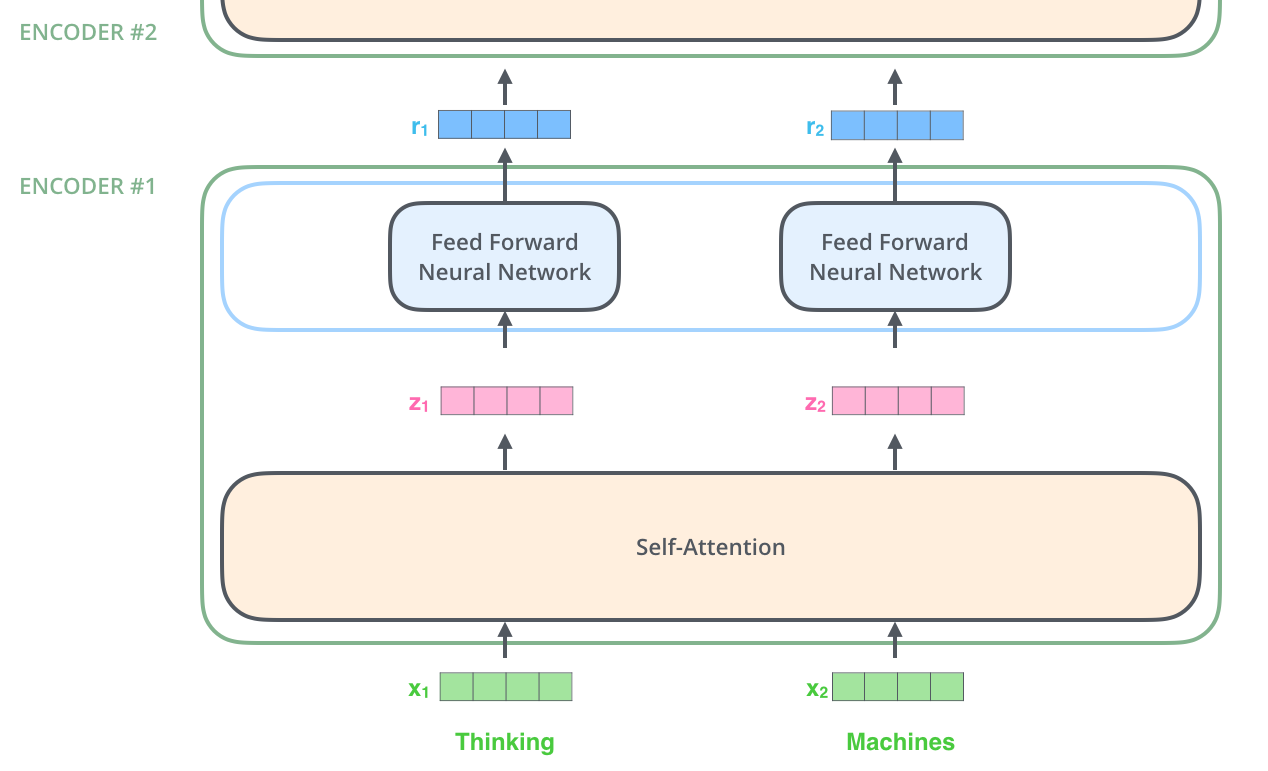
\includegraphics[scale=0.1]{img/transf2.png}
			\end{center}
		\end{figure}
	\end{frame}
	
	\begin{frame}
	\frametitle{Трансформеры. Self Attention}
		\begin{figure}[H]
			\begin{center}
				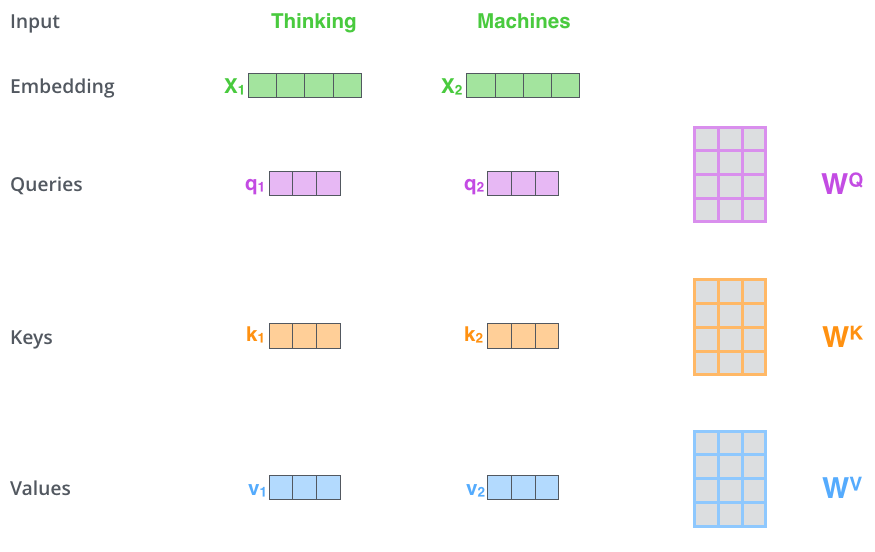
\includegraphics[scale=0.15]{img/transf3.png}
			\end{center}
		\end{figure}
		
		\begin{figure}[H]
			\begin{center}
				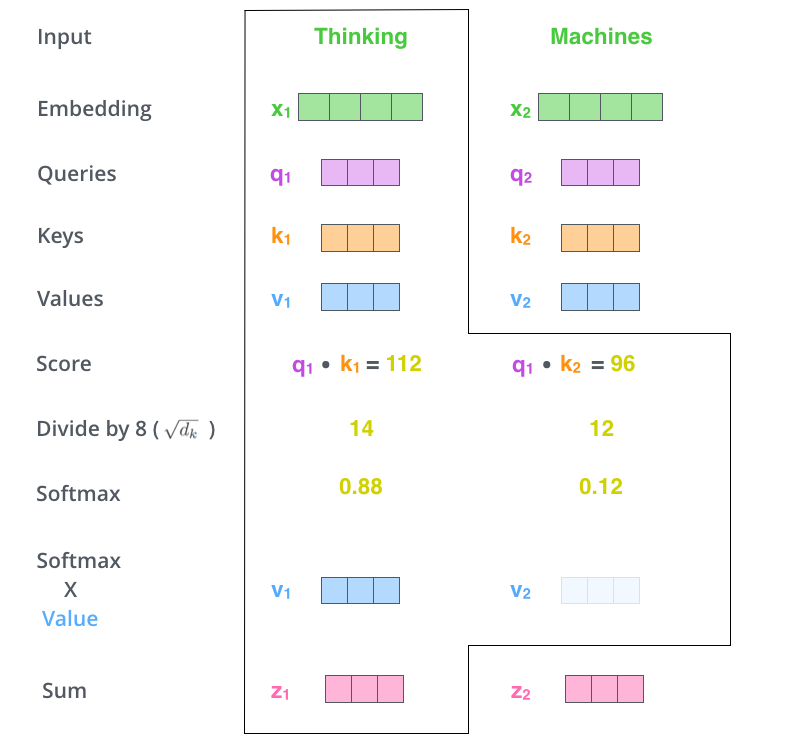
\includegraphics[scale=0.15]{img/transf4.png}
			\end{center}
		\end{figure}
	\end{frame}
	
	\begin{frame}
	\frametitle{Трансформеры. Self Attention}
		\begin{minipage}{0.35\textwidth}
			\centering
			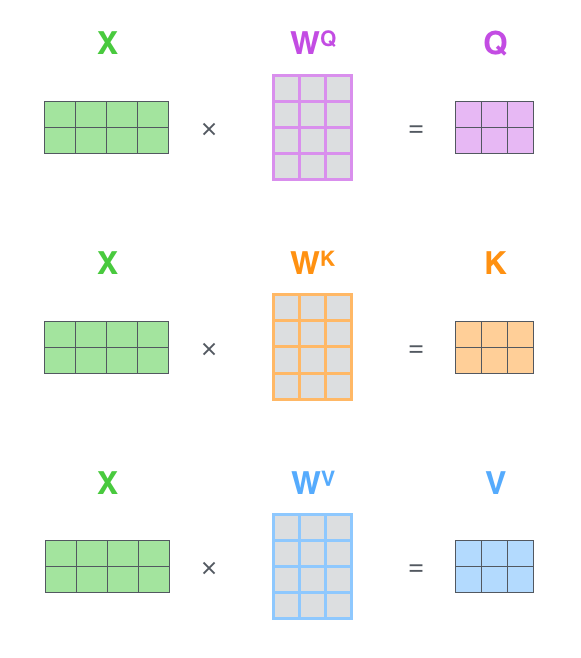
\includegraphics[scale=0.15]{img/self-attention.png}
		\end{minipage}\hfill
		\begin{minipage}{0.6\textwidth}
			\centering
			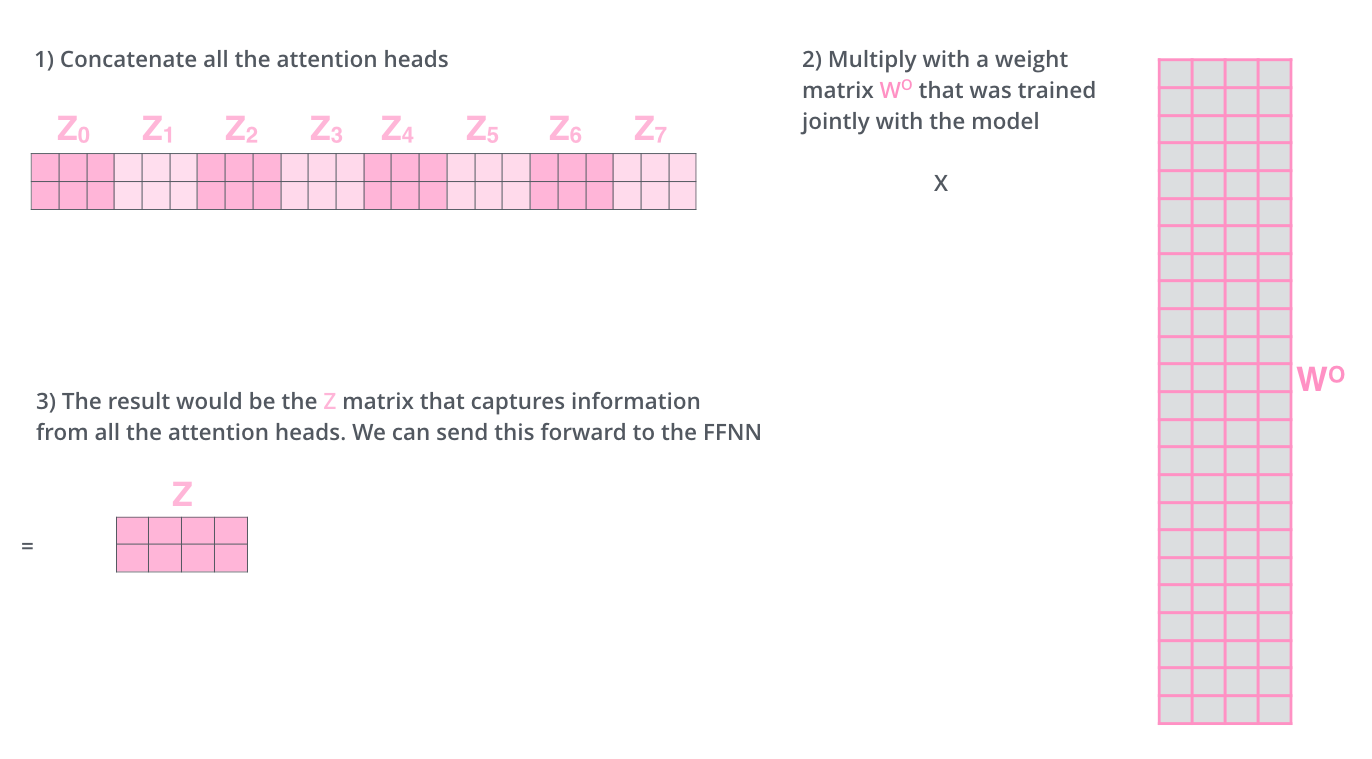
\includegraphics[scale=0.15]{img/multi-head-att.png}
		\end{minipage}
		\begin{figure}[H]
			\begin{center}
				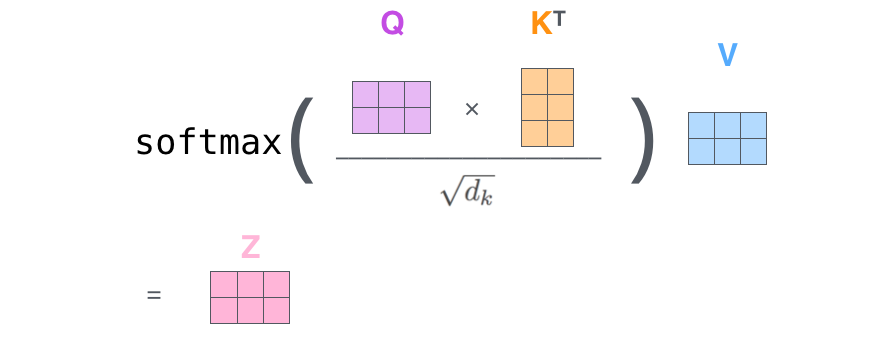
\includegraphics[scale=0.2]{img/self-attention2.png}
			\end{center}
		\end{figure}
	\end{frame}
	
	\begin{frame}
	\frametitle{Трансформеры. Self Attention}
		\begin{figure}[H]
			\begin{center}
				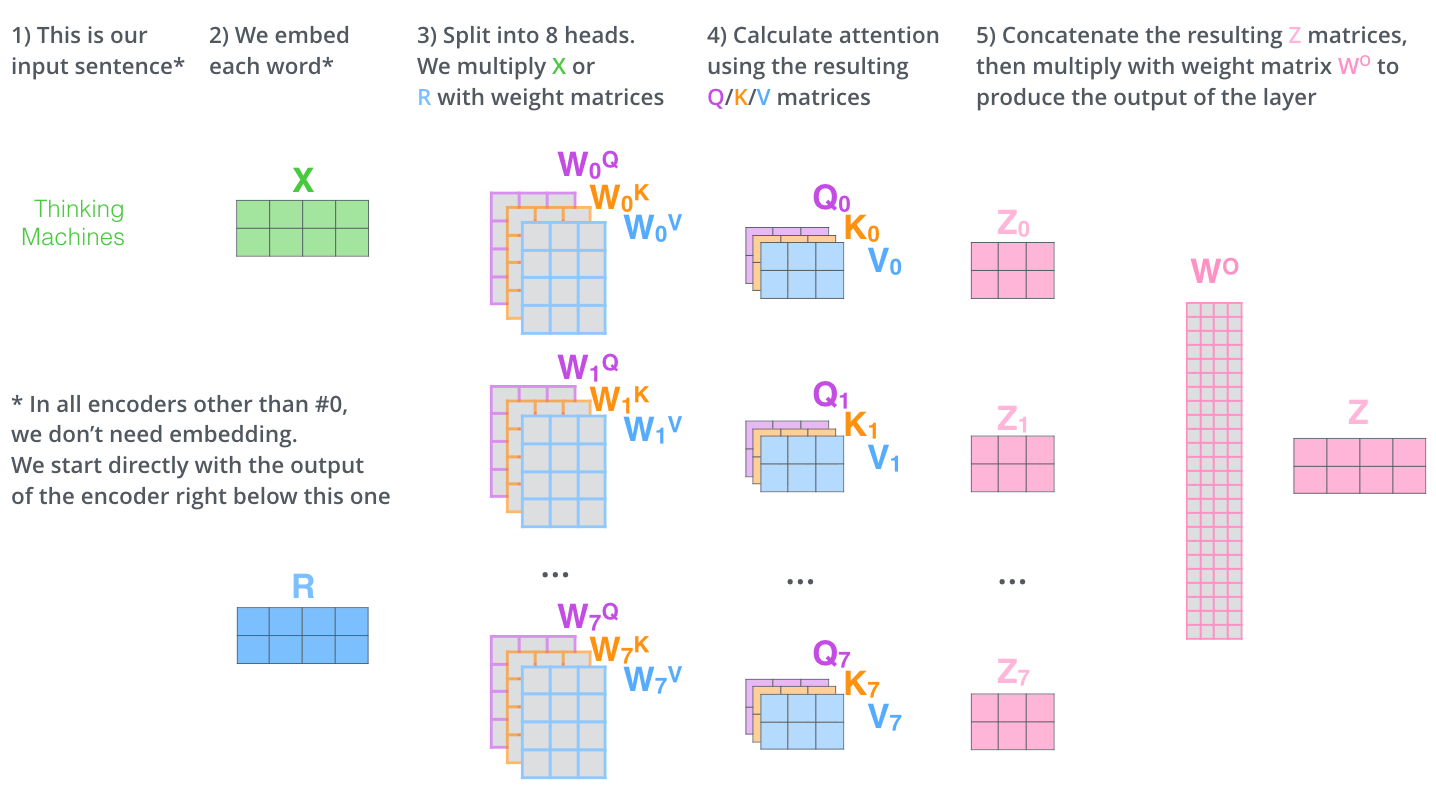
\includegraphics[scale=0.15]{img/att-all.png}
			\end{center}
		\end{figure}
		\begin{figure}[H]
			\begin{center}
				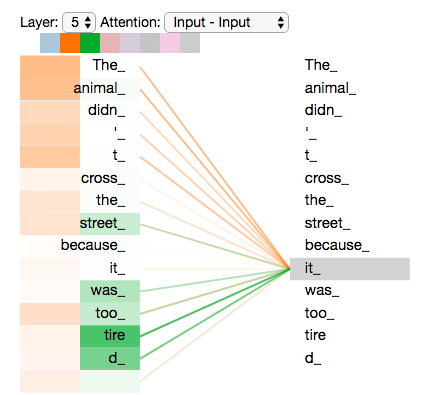
\includegraphics[scale=0.2]{img/att-ex.png}
			\end{center}
		\end{figure}
	\end{frame}
	
	\begin{frame}
	\frametitle{Трансформеры. Positional encoding}
		Можем закодировать информацию о позиции слова следующим образом:
		
		$\mbox{PE}_{pos, 2i}=\sin(pos/10000^{2i/d_{model}}),$
		$\mbox{PE}_{pos, 2i+1}=\cos(pos/10000^{2i/d_{model}})$,
		
		после чего можем добавить получившийся энкодинг к эмбеддингам.
		\begin{figure}[H]
			\begin{center}
				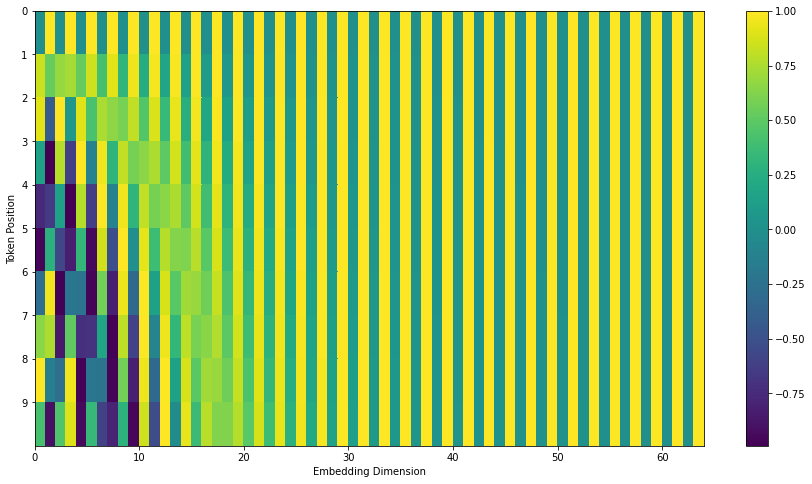
\includegraphics[scale=0.3]{img/pos-enc.png}
			\end{center}
		\end{figure}
	\end{frame}
	
	\begin{frame}
	\frametitle{Трансформеры. Masked Attention}
	Входная последовательность декодера маскируется таким образом, что Attention Score для каждого токена считается только с токенами, которые находятся перед ним. Для encoder--decoder attention матрица Q берется из декодера, а матрицы K и V --- из энкодера.
		\begin{figure}[H]
			\begin{center}
				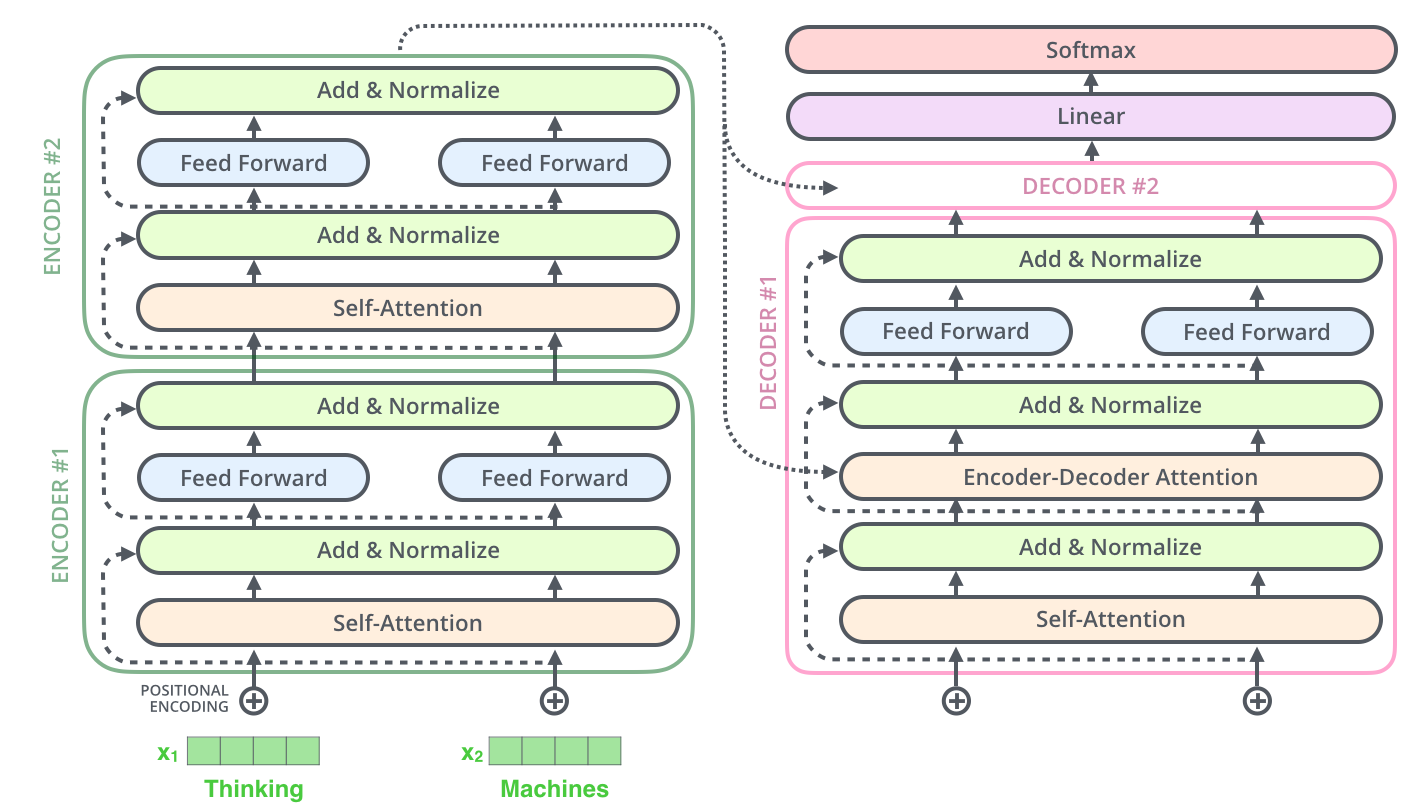
\includegraphics[scale=0.18]{img/transf.png}
			\end{center}
		\end{figure}
	\end{frame}
	
	\begin{frame}
	\frametitle{Трансформеры. Train \& Inference}
		Последний линейный слой преобразовывает выход декодера из размерности (batch size, sequence lenght, embedding size) в размерность (batch size, sequence length, vocabulary size), после чего считается 
		
		$Loss = -\sum\limits_{t=1}^{T}\log(p_{y_t}).$
		
		Для прогнозирования подаем декодеру <SOS> (start of sequence) токен, после чего добавляем ко входу декодера предсказанный токен и повторяем процесс до того, как декодер выведет <EOS> (end of sequence) токен. 
		\vspace{0.3cm}
		
		Преимущества архитектуры: 
		\begin{enumerate}
			\item Работает быстрее, так как нет рекуррентных блоков.
			\item Много вычислений, которые можно распараллелить. 
		\end{enumerate}
	\end{frame}
	
	\begin{frame}
		\frametitle{BERT (Bidirectional Encoder Representations from Transformers)}
		\begin{figure}[H]
			\begin{center}
				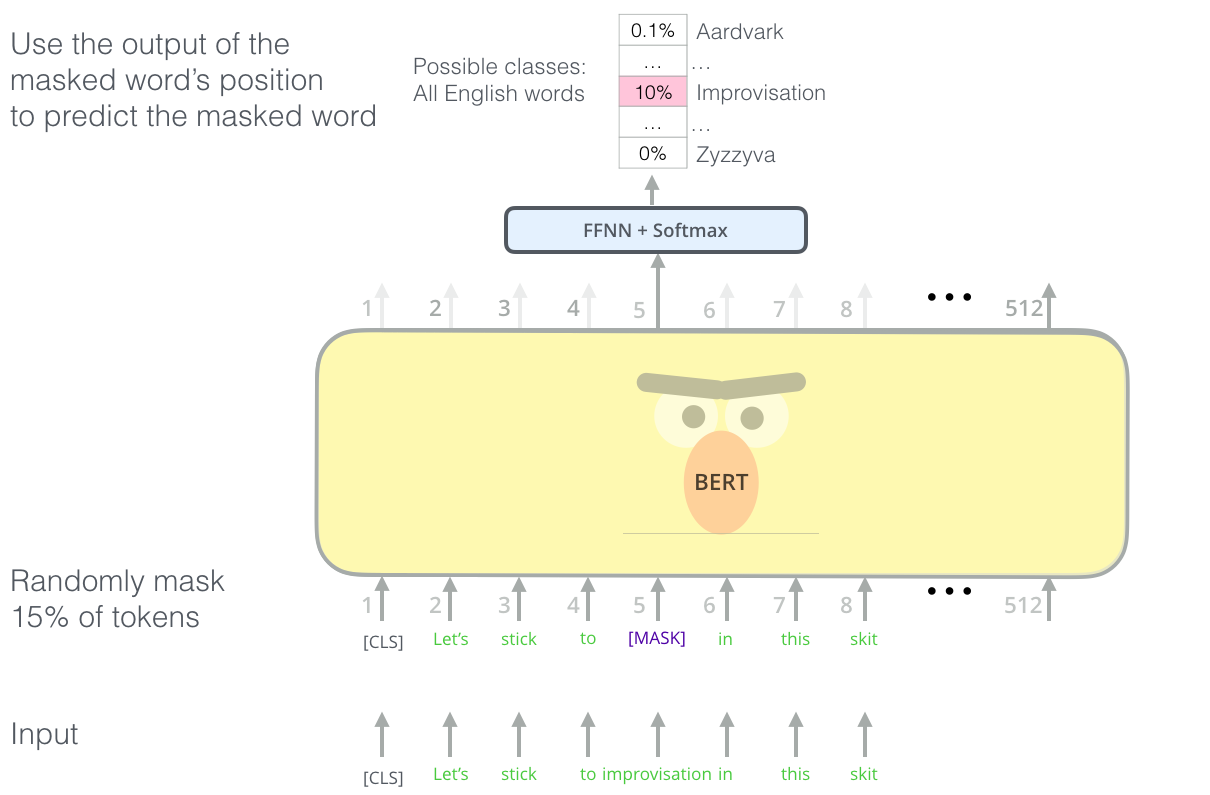
\includegraphics[scale=0.12]{img/bert.png}
			\end{center}
		\end{figure}
		\begin{figure}[H]
			\begin{center}
				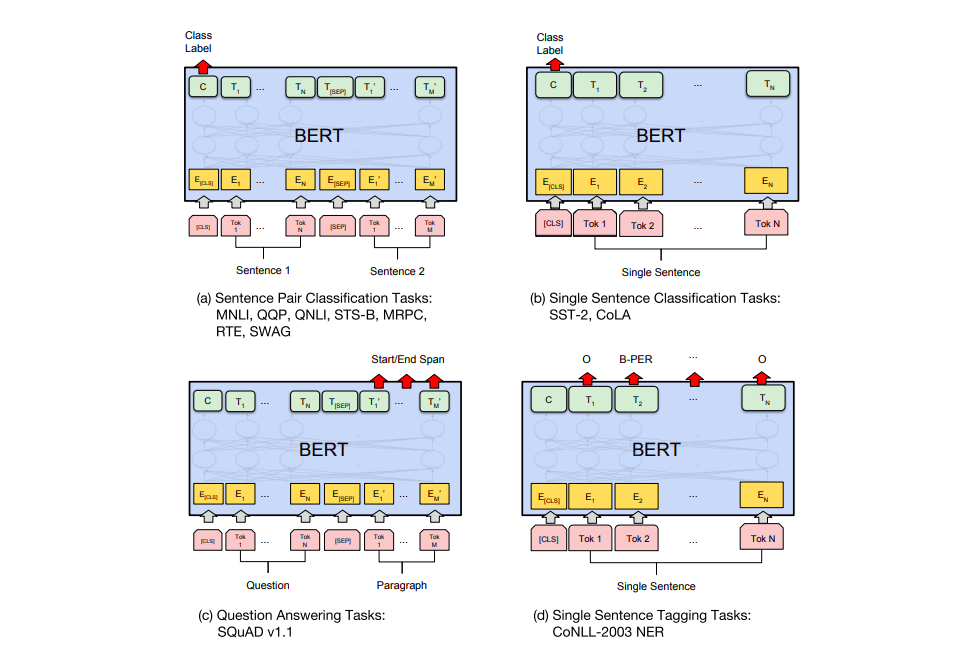
\includegraphics[scale=0.15]{img/bert2.png}
			\end{center}
		\end{figure}
	\end{frame}
	
	\begin{frame}
	\frametitle{Transfer Learning}
		\begin{figure}[H]
			\begin{center}
				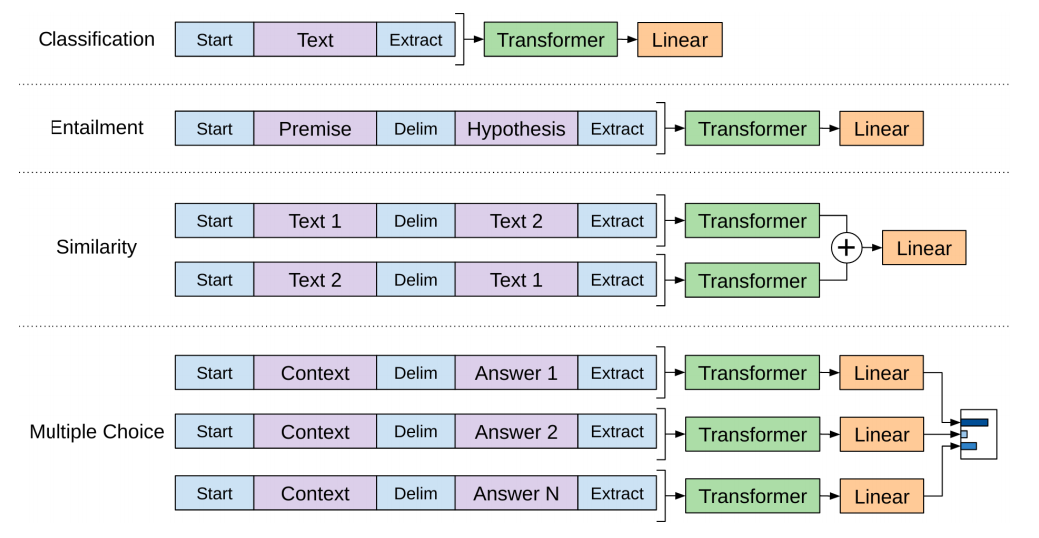
\includegraphics[scale=0.3]{img/gpt-tuning.png}
			\end{center}
		\end{figure}
	\end{frame}
	
\end{document}